\documentclass[a4paper,11pt]{article}
\usepackage{fullpage}

\usepackage{subfigure}
\usepackage{enumitem}
\usepackage{graphicx}
\usepackage{amsmath}
\usepackage{pgf}
\usepackage{float}
\newtheorem{definition}{Definition}
\let\cleardoublepage\clearpage
\usepackage{todonotes}
\newcommand{\TJ}[1]{\todo[color=green!50]{\sf \textbf{TJ:} #1}}
\newcommand{\TAP}[1]{\todo[inline,color=red!50]{\sf \textbf{TAP:} #1}}
\newcommand{\MQ}[1]{\todo[inline,color=blue!50]{\sf \textbf{MQ:} #1}}



\RequirePackage{multidef}
\RequirePackage{xspace}
\multidef[prefix=bb]{\mathbb{#1}\xspace}{A-Z,One->1}
\multidef{\textsf{#1}}{Actors,Network,Synchronization,Mailboxes,Communications,mailbox,communication,Mutexes}
\multidef{\textsf{\textit{#1}}}{send,receive,mutexlock->MutexAsynLock,mutexunlock->MutexUnlock,mutexwait->MutexWait,mutextest->MutexTest, localcomputation->LocalComputation, asynsend->AsynSend, asynreceive->AsynReceive, test->Test, wait->Wait}


\title{Formal Semantics of the SimGrid Simulator}
\begin{document}
\maketitle

This document tries to formally express the semantic of applications that can be executed in SimGrid, such as MPI applications. The long term goals is to find better reduction algorithms for MPI applications in Mc SimGrid, the model-checker embedded within the SimGrid framework.

\medskip

SimGrid is a simulator of distributed applications. Several user interfaces are proposed, ranging from the classical and realistic MPI formalism, to less realistic simgrid-specific APIs that ease the expression of theoretical distributed algorithms. These user interfaces are built upon a common interface, that is implemented either on top of a performance simulator, or on top of a model-checker exploring exhaustively all possible outcomes from a given initial situation.

\centerline{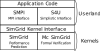
\includegraphics[scale=.6]{simgrid-architecture.pdf}}

The distributed application is represented in SimGrid as a set of \textbf{actors}, representing  
processes or threads of real applications, or MPI ranks. These actors  interact with each other either through message passing, or with classical synchronization objects (such as mutexes or semaphores), or through executions on CPUs and read/write  operations on disks.

Even if it simulates distributed applications, SimGrid proposes a shared memory model: all actors share the same memory space. Most of the simulated applications enforce a memory separation by not using any program global variables but only variables that are local to each actor (this privatization is automatically handled at compilation time for MPI programs). Enforcing the memory separation at application level allows the kernel to deal with shared-memory and distributed-memory primitives in the same way.

From the formal point of view, a major advantage of the SimGrid framework is that all user interfaces are implemented on top of a very small amount of kernel primitives.
In this document, we are interested in formalizing these operations and their inter-dependencies, that will be useful for partial-order reduction methods  in model-checking.

Once we defined all possible events in section 1, we need to define an event system. For that, we need:
\begin{itemize}
\item Causality relation, which can be derived from happens-before relation.
\item Conflict relation
\item Independence relation: I(e1,e2) means that there is no causality chain between e1 and e2.
\end{itemize}

\section{System State Definition}
A distributed system is a tuple $P=\langle \Actors, \Network, \Synchronization \rangle$ in which  $\Actors$ = $\{ A_1, A_2, ... A_n\}$ is a set of $n$ actors. Actors do not have a global shared memory nor a global clock. The execution of an actor $A_i$ consists of an alternate sequence of local states and events (transitions)
$s_{i,0}\xrightarrow{\text{$e_0$}} s_{i,1} \xrightarrow{\text{$e_1$}}s_{i,2} ... \xrightarrow{\text{$e_{n-1}$}}s_{i,n}$ (firing $e_i$ from local state $s_{i}$, the local state of the actor $A_i$ changes from $s_i$ to $s_{i+1}$).
All the events in one actor are totally ordered by the causal relation (see below) \TJ{this will be discussed later ?}. \Network~is considered as a subsystem in the program P, and it provides facilities for the \Actors~ able exchange messages with each other. \Synchronization~consist of several mechanisms to synchronize actors when they are accessing shared resources. 

\subsection{Network Subsystem}
The state of the network subsystem is defined as a pair $\langle \Mailboxes, \Communications \rangle$, where \begin{itemize}[noitemsep]
\setlength{\itemsep}{3pt}
\item $\Mailboxes = \{ \mailbox_1, \mailbox_2, ... \mailbox_m \}$ is a set of $m$ mailboxes, each $\mailbox_i$ is an infinite queue storing $\send$ and $\receive$ requests of agents, it is considered as a rendez-vous
where $\send$ and $\receive$ requests meet. For a given mailbox, corresponding requests are stored with a FIFO policy. It means that when a $\send$ request coming to the mailbox, the oldest $\receive$ is selected to combine with the coming $\send$, producing a ready communication in \Communications~ (the same process for receive requests). Hence, at the same time there are only one kind of pending requests: send or receive requests. The state of the mailbox is indicated by the pending $\send$ or $\receive$ requests. Therefor, the mailbox's state is changed if there is an actor sending a $\send$ or $\receive$ request to it. 
\item $\Communications$ is a set of individual communications, each of them describing a data exchange  between two actors.  A $\communication$ with the "ready" status is formed when a $\send$ request matches with a $\receive$ request in a particular mailbox. While a "ready" \communication~ is ready for exchanging data between two actors, a communication whose status is "\send" or "\receive" is waiting for the supplement information to create a complete communication (ready communication)
\end{itemize}
Four events are defined in \Network~ subsystem to support actors communicate with each other. They are \asynsend, \asynreceive, \wait~ and \test. An actors start a communication by firing a \asynsend~ or \asynreceive; however, data are really exchanged betwen two actors because of firing \wait~ or \test.
\begin{itemize}[noitemsep]
\setlength{\itemsep}{3pt}
\item An actor drops an asynchronous \send~ request to a particular mailbox by firing an \asynsend~ event. If there are pending \receive~ requests in the mailbox, the \send~ request will be matched with the oldest receive request to form a \communication~ with "ready" status in the \Communications. In the other hand, there is no pending receive in the mailbox, the request is stored in the mailbox and a \communication~ is still created in the \Communications~ with a "send" status.  Similarly, actors use \asynreceive~ to post an asynchronous receive on a mailbox; the way a receive request is processed is the same as the way a send request is treated. 

\item Although communications are established in the \Communications~ by the combination of \send~ and \receive~ requests, data are really transferred between actors by firing \test~ or \wait. \test~ returns either true or false depending on the status of the \communication~ what the \test's actor want to test. If the status is "ready" or "done", it returns true, otherwise false is given. As stated, data exchange is performed in \test~ command. In the case where the status is "ready", data is copied from the souse actor to the destination actor, and the status of the communication is assigned to "done". Similarly, \wait~ event has the same function in transferring data, but  it does not return any values, and like \mutexwait, it can blocks it's actor if the \communication~ is not ready for being processed.   
\end{itemize}

\subsection{Synchronization subsystem}
The state of the \Synchronization~ subsystem is defined by \Mutexes
\begin{itemize}[noitemsep]
\setlength{\itemsep}{3pt}
 \item 
  $\Mutexes$ = $\{m_1, m_2 ... m_k \}$ is a set of k asynchronous mutexes. The $\Mutexes$ are used to synchronize the actors. An actor $A_i$ declares it's interest on a mutex $m_j$ by executing the action $\mutexlock(A_i,m_j)$~  while the mutex remembers that interest by adding the id of the actor to it's waiting queue. This queue also follows a FIFO policy. An actor is considered the {\em owner} of a mutex if it is the first in the mutex's waiting queue while the others in the queue are [\em waiting] actors. We say that a mutex $m$ is {\em busy} if there is at least one actor in it's waiting queue, otherwise it is {\em free}.
 \end{itemize}

 In this model mutexes are asynchronous, similar to communication, in the sense that requesting a mutex is not blocking. 
 In the synchronization subsystem, there are four events  allowing actors to interact with the \Mutexes, namely \mutexlock, \mutexunlock, \mutexwait~ and \mutextest, where  
 \begin{itemize}[noitemsep]
\setlength{\itemsep}{3pt}
 \item $\mutexlock(A_i,m_j)$~ is executed by an actor $A_i$ when the actor wants to acquire a mutex $m_j$. After firing \mutexlock, the id $i$ of the actor will be added to the tail of the mutex's queue. If the mutex was free, the actor becomes the owner of the mutex, and to help the actor identify which mutexes it has asked for, the mutex's id $j$ is added to it's requests set \TJ{add this in the actors state?}. Unlike classical mutexes, when an actor is waiting for a mutex, it is not blocked.
\item \mutexunlock~ is used to remove an interest on a mutex by an actor. Either the actor is the owner or not, this command can be fired by the mutex, deleting the id of the actor from the mutex's queue and removing the mutex's id from actor's request set. 
\item An actor can check if it is the owner of a mutex that he has previously asked for access to (id of the mutex is included in the actor's request set). To realize this, it can use the \mutextest~action, returning true if the id of the actor is the first element of the mutex's waiting queue, otherwise the returned value is false. While a \mutextest~ can be fired at any time, a \mutexwait~ can only be executed by an actor when the actor owns the mutex. Hence, a waiting actor can be blocked when trying to execute \mutexwait. 
 \end{itemize}

\subsection{Summary}
Actor = local state (containing variables and PC) + program (sequence of events) 

\noindent\centerline{\begin{tabular}{|c||c|c|}\hline
 \textbf{Subsystem}&\Network&\Synchronization\\\hline\hline
 %
 \textbf{Resource}&Mailbox& Mutex\\\hline
 %
 \textbf{Activity}&Communication&Request\\\hline
 %
 &Send=\asynsend+\wait&Lock=\mutexlock+\mutexwait\\
 \textbf{Events}&Recv=\asynreceive+\wait&\mutexunlock\\
  &\test&\mutextest\\\hline
\end{tabular}}

\section{Happened-before relation}
\begin{figure}[H]
	\label{fig:cycle_dependency}
	\begin{center}
		%\includegraphics[width=7cm,height=6cm]{example.jpg}
		\centerline{\includegraphics[scale=.8]{example.pdf}}

	\end{center}
	\caption{A MPI program with a potential deadlock}
\end{figure}
In SimGrid, events are atomic and events in the same actor are totally ordered, but events in the whole system are partially ordered (partial order relation).  Hence, there are different instances (runs) of the system, and the relation between events are  considered in a given instance. A global state is defined as a set of local states of the actors, and states of the $Mailboxes$ and states of the $Mutexes$. State $S_0$ is used to present the initial state of the system. In the initial state all the mailboxes are empty, all mutexes are free, local variables are initialized. Function execute($S_i$,t)  gives the next global state after executing transition t in the state $S_i$ while function $getEnabled(S_i)$
gives all the enabled transitions at state $S_i$.\\

 To adapt to the reality, happened-before relation in SimGrid is flexible. Let's look at an example in Figure~\ref{fig:cycle_dependency}. A MPI program including two processes, and process P0 sends a massage to process P1 (doted line). Before receiving  the massage from P0, P1 also sends a massage to P0. At first glance, we may think that there is a deadlock in the program since there is a dependency cycle. However, in practice, depending on the size of the massages exchanged by the processes, the deadlock may appears or not. MPI\_Send and MPI\_Receive are blocking events in MPI, but they may or may not block. MPI\_Send is ambiguously define, it will not return until the buffer passed to it can be reused. For sending small enough massages, those massage eagerly sent before the calling MPI\_Receive from receiving processes (eager protocol). Hence, MPI\_Sends are not blocked until matching MPI\_Receive have been posted. Actually, if the massages are small, MPI can easily find spaces in internal storage to save them before they are really sent. On the other hand, working with large massages, blocking communications are used, MPI\_Sends must wait for matching MPI\_Receives. Therefor, the scenario in Figure~\ref{fig:cycle_dependency} may or may not has a deadlock. SimGrid covers both cases, users can chose optionally two modes detecting or not deadlocks in the same situation with the above scenario. This conversion can be done easily by switching between two happened\_before relations definition.    
  \begin{definition}
  	\label{def:happedBefore1}
  The happened-before relation  denoted by  $\rightarrow $ can be defined based on two relations precede and causality: \begin{itemize}
  	\item Precede $ \prec$ :  Two events e and f in the same actor $A_i$, e $ \prec$ f if the occurrence of e precedes the occurrence of f in the actor $A_i$  
  	\item Causality $<$ : Event e is the \asynsend~ or \asynreceive~ event of actor $A_i$, event f is the Wait event of the actor $A_j$,  e $<$ f if e and f concerns the same communication request.
  	\item The ‘happened before’ is a transitive relation including precede and causality relations. 
  \end{itemize}\end{definition} 
  
 \begin{figure}[H]
\label{fig:hapend_before}
\subfigure[deadlock]{
		\includegraphics[width=7cm,height=7cm]{deadlock.pdf}
	}
\hfill
\subfigure[dealock free]{
\includegraphics[width=7cm,height=7cm]{deadlockFree.pdf}
	}
\caption{Happened- before relations between events}
\end{figure}

The diagram in Figure~\ref{fig:hapend_before}(a) illustrates happened\_before relations (denoted by arrow lines) between events in the program based on Definition~\ref{def:happedBefore1}. In SimGrid a MPI\_Send is simulated by a \asynsend~ and a \wait~ while a MPI\_Receive consist of a \asynreceive~ and a \wait. Obviously, there is a happened\_before relation cycle in the diagram; the cycle includes the first Wait and \asynreceive~ of P0, the first Wait and the \asynreceive~ of P1. The existing of cycle leads to a deadlock in the program. In the case we do not want to capture the deadlock, Definiton~\ref{def:happedBefore2} is used.

\begin{definition}
	  	\label{def:happedBefore2}
	The happened-before relation  denoted by  $\rightarrow $ can be defined based on two relations precede and causality: \begin{itemize}
		\item Precede $ \prec$ :  Two events e and f in the same actor $A_i$, e $ \prec$ f if the occurrence of e precedes the occurrence of f in the actor $A_i$  
		\item Causality $<$ : Event e is the \asynsend~ event of actor $A_i$, event f is the \wait~ event of the actor $A_j$,  e $<$ f if e and f concerns the same communication request.
		\item The ‘happened before’ is a transitive relation including precede and causality relations. 
	\end{itemize}\end{definition} 

Using Definition~\ref{def:happedBefore2} and presenting the happened\_before relation between events of the program in Figure~\ref{fig:hapend_before}(b), we can see that there are no any cycle, then the program is deadlock-free.

The happened-before relation is not a total order on the events, two events may not related by a happened-before relation. In that case, we say that they are concurrent denoted by the symbol $\parallel$. For example, in the above figures, since $\neg$(\asynsend~ of P0 $<$ \asynsend~ of P1) and $\neg$(\asynsend~ of P0 $ \prec$  \asynsend~ of P1 ) then \asynsend~ of P0 $\parallel$ \asynsend~ of P1.  

\section{MPI Implementation}
TODO: explain here how MPI is implemented on top of the previously described API
%\newpage

%\nocite{*}	  	
%\bibliographystyle{alpha}
%\bibliography{report}
	
\end{document}